\documentclass[letterpaper,12pt]{article}
 \usepackage[utf8]{inputenc}
\usepackage[T1]{fontenc}
% \usepackage[latin9]{inputenc}
\usepackage{amstext}
\usepackage{amsmath}
\usepackage{amssymb}
\usepackage{graphicx}
\usepackage{geometry}
\usepackage{tikz}
\usepackage{esint}
\usepackage{caption}
\usepackage{subcaption}
\usepackage{enumerate}

\geometry{
 letterpaper,
%  total={210mm,297mm},
 left=1.25in,
 right=1.25in,
 top=1.5in,
 bottom=0.5in,
 }
 
 \begin{document}
  \begin{picture}(0,0)
\put(114,-10){
\includegraphics[width=6cm]{Images/un_logo.eps}}
\end{picture}
\begin{center}
\textbf{
 FACULTAD DE INGENIER\'IA\\
 Vicedecanatura Acad\'emica\\
 POSGRADOS \break
  \newline
 PROPOSAL SUBMISSION
}

\end{center}
\vspace{30pt}

% •Título preliminar
% •Justificación
% •Estado del arte
% •Definición del problema
% •Metodología
% •Cronograma aproximado
% •Sectores de impacto de la investigación
% •Referencias bibliográficas 

%checkboxes
\begin{tabular}{l c l c}
 DOCTORAL THESIS: & \framebox[0.5cm][c]{x} & MASTER THESIS: & 
\framebox[0.5cm][c]{}\\
 MASTER FINAL WORK: & \framebox[0.5cm][c]{} & SPECIALIZATION FINAL WORK: & 
\framebox[0.5cm][c]{}\\ 
\end{tabular}
\vspace{20pt}
 \begin{enumerate}
  \item \textbf{BIDDER:} Robinson Andr\'es Jaque Pirab\'an \qquad\qquad 
\textbf{ID:} 80190790
  \item \textbf{PROGRAM:} Phylosophy Doctoral in Computer Science and Systems 
Engineering
  \item \textbf{ADVISOR:} Fabio Augusto Gonz\'alez Osorio\\
  \textbf{DEPARTMENT:} Computer Science and Industrial Engineering
  \item \textbf{TITLE: Kernel Tensor Factorization }%check
  \item \textbf{AREA:} Computer Science
  \item \textbf{LINE OF RESEARCH:} Machine Learning
  \item COMMENTARY WITH ADVISOR APROVAL
  \vspace{120pt}
% % 14. COMENTARIO CON VISTO BUENO DEL DIRECTOR: (calificar los siguientes 
% aspectos: organización, pertinencia, relevancia y originalidad).
  \item BIDDER SIGNATURE 
%  
%  Robinson Andr\'es Jaque Pirab\'an
% % 15. FIRMA DEL PROPONENTE
  \vspace{60pt}
  \item SIGNATURE OF ADVISOR
  \vspace{60pt}
 % 16. FIRMA DEL DIRECTOR (ASESORES)
 % 17. FECHA  
  \end{enumerate}  
  
%   \item \textbf{BACKGROUND AND JUSTIFICATION:}\\
  
% 5. ANTECEDENTES Y JUSTIFICACIÓN: (Indicar los desarrollos previos, 
% circunstancias y condiciones que llevaron a la conclusión de la necesidad y 
% conveniencia del proyecto)

%  \item \textbf{PROBLEM STATEMENT:}\\
% 6. IDENTIFICACIÓN DEL PROBLEMA: 


\clearpage

%Portada

\clearpage

\tableofcontents

\newpage

\section{Introduction}

Data-driven unsupervised learning has been establishing itself as a critical component of scientific discovery in domains ranging from astrophysics to social sciences and computational journalism. It manifests itself, among many forms, through modeling, machine learning, data mining, pattern recognition, data analytics, anomaly detection, and visualization. Nowaday, have rised a high volume of multiway data since the widespread use of multisensor technology and natural multiway structure of multimedia data, such as images, video or audio. This context have highlighted the limitations of standard flat-view matrix models and the necessity to move toward more versatile data analysis tools. In that sense, multiway analysis is of paramount importance. Data analysis techniques using tensor decompositions are shown to have great flexibility in the choice of constraints which match data properties and extract more general latent components in the data than matrix-based methods.

\subsection{Basics of tensors}

Tensors are multidimensional arrays, i.e. an $N$-way or $N$-order tensor is an element of tensor product of $N$ vector spaces, each of which has its own coordinate system. A first order tensor is a vector, a second order tensor is a matrix, tensors of higher order are called high-order tensors. The order (ways or modes) of a tensor is the number of dimensions. Figure \ref{fig:3tensor} represents a 3-order tensor $\mathcal{X}\in\mathbb{R}^{I\times J\times K}$.

\begin{figure}[!ht]
\centering
 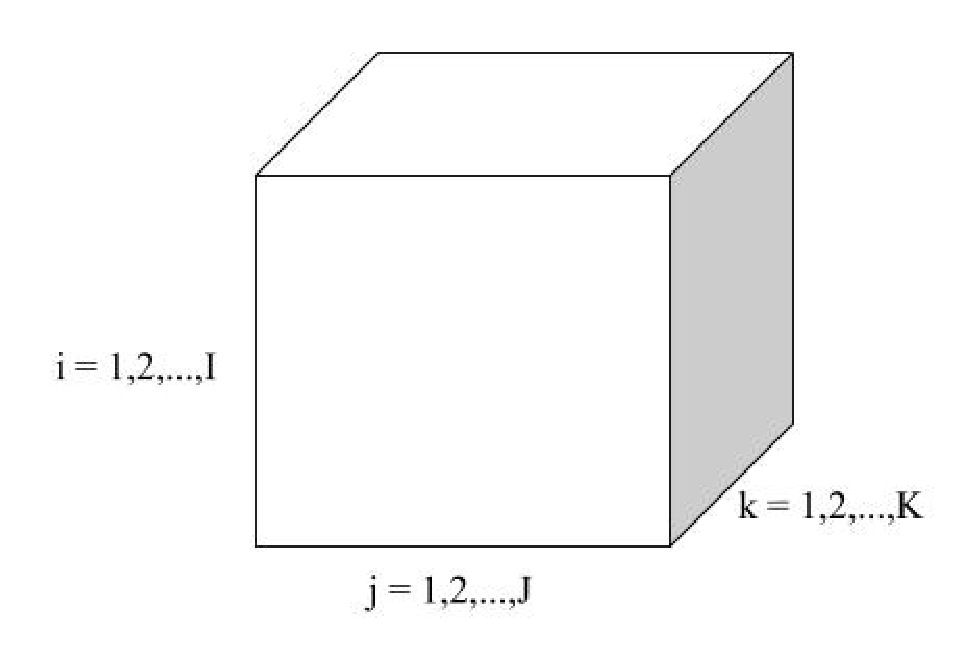
\includegraphics[scale=0.4]{Images/3rd-order_tensor.eps}
 \caption{Third-order tensor}\label{fig:3tensor}
\end{figure}

\textit{Fibers} are defined by fixing every index by one. In a third-order tensor a column is a mode-1 fiber, denoted by $x_{:jk}$; a row is a mode-2 fiber, denoted by $x_{i:k}$; while a tube is a mode-3 fiber, denoted by $x_{i:k}$. \ref{fig:3tensor-fibers} shows a fibers representation in 3rd-order tensor.

\begin{figure}[!ht]
 \centering
 \begin{subfigure}[b]{0.29\textwidth}
  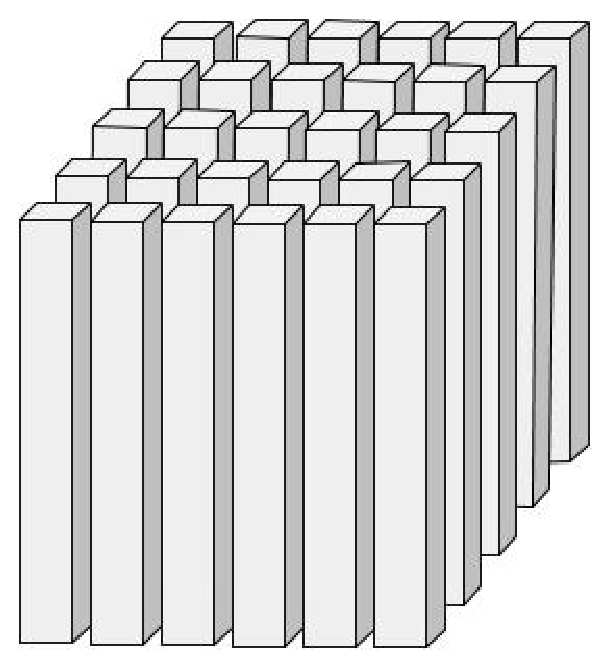
\includegraphics[width=\textwidth]{Images/3rd-order-tensor-fiber_mode-1.eps}
  \caption{columns}\label{fig:3tensor-columns}
 \end{subfigure}
 \begin{subfigure}[b]{0.33\textwidth}
  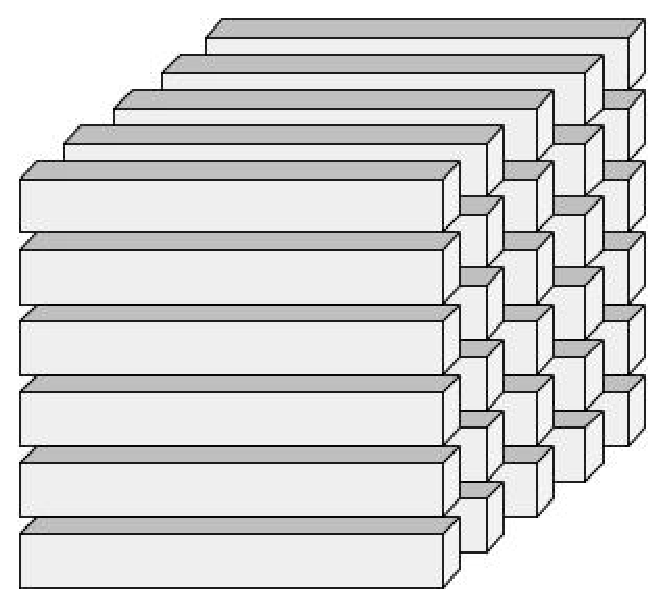
\includegraphics[width=\textwidth]{Images/3rd-order-tensor-fiber_mode-2.eps}
  \caption{rows}\label{fig:3tensor-rows}
 \end{subfigure}
 \begin{subfigure}[b]{0.33\textwidth}
  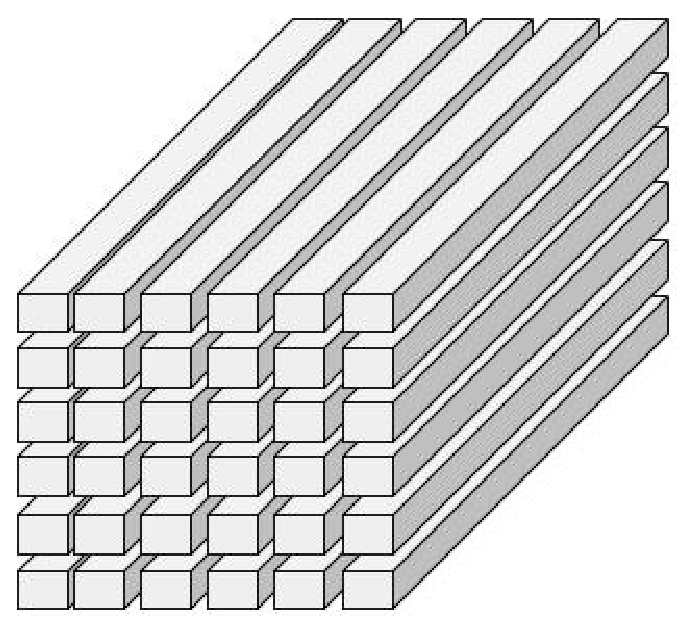
\includegraphics[width=\textwidth]{Images/3rd-order-tensor-fiber_mode-3.eps}
  \caption{tubes}\label{fig:3tensor-tubes}
 \end{subfigure}
\caption{3rd-order tensor fibers}\label{fig:3tensor-fibers}
\end{figure}

\textit{Slices} are two-dimensional sections of a tensor defined by fixing two indexes. For instance, slices of 3rd-order tensor $\mathcal{X}$ are denoted by $X_{i::}$ (horizontal), $X_{:j:}$ (lateral) and $X_{::k}$ (frontal) and we ilustrate them in figure \ref{fig:3tensor-slices}.

\begin{figure}[!ht]
 \centering
 \begin{subfigure}[b]{0.29\textwidth}
  
\includegraphics[width=\textwidth]{Images/slices-frontal.eps}
  \caption{Frontal slices}\label{fig:3tensor-frontalslices}
 \end{subfigure}
 \begin{subfigure}[b]{0.33\textwidth}
  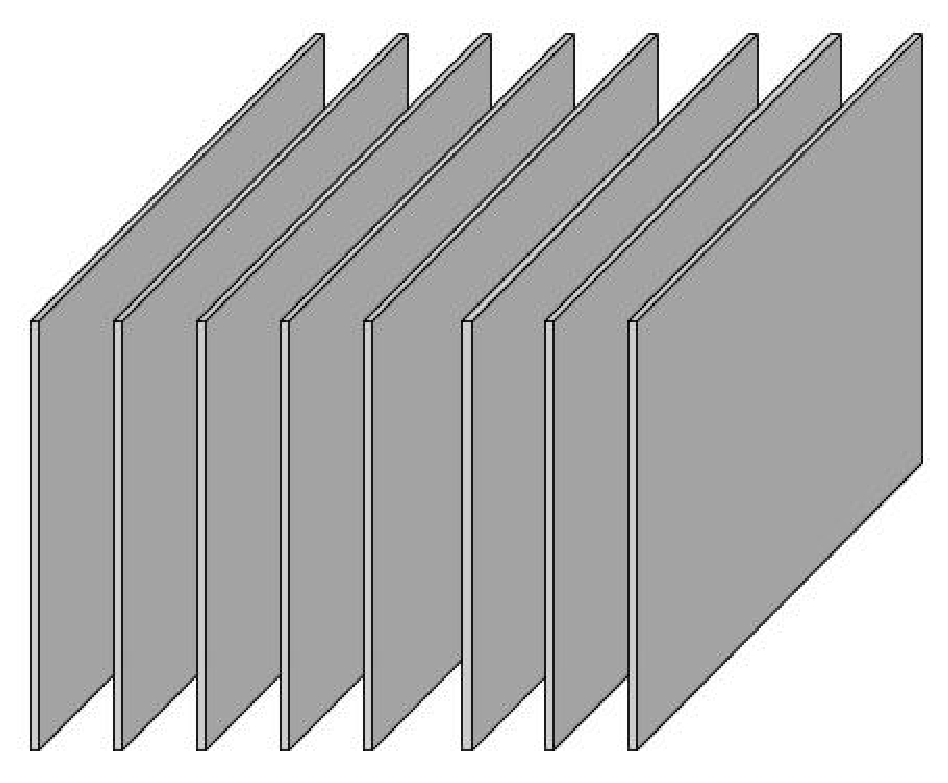
\includegraphics[width=\textwidth]{Images/slices-horizontal.eps}
  \caption{Horizontal slices}\label{fig:3tensor-horizontalslices}
 \end{subfigure}
 \begin{subfigure}[b]{0.33\textwidth}
  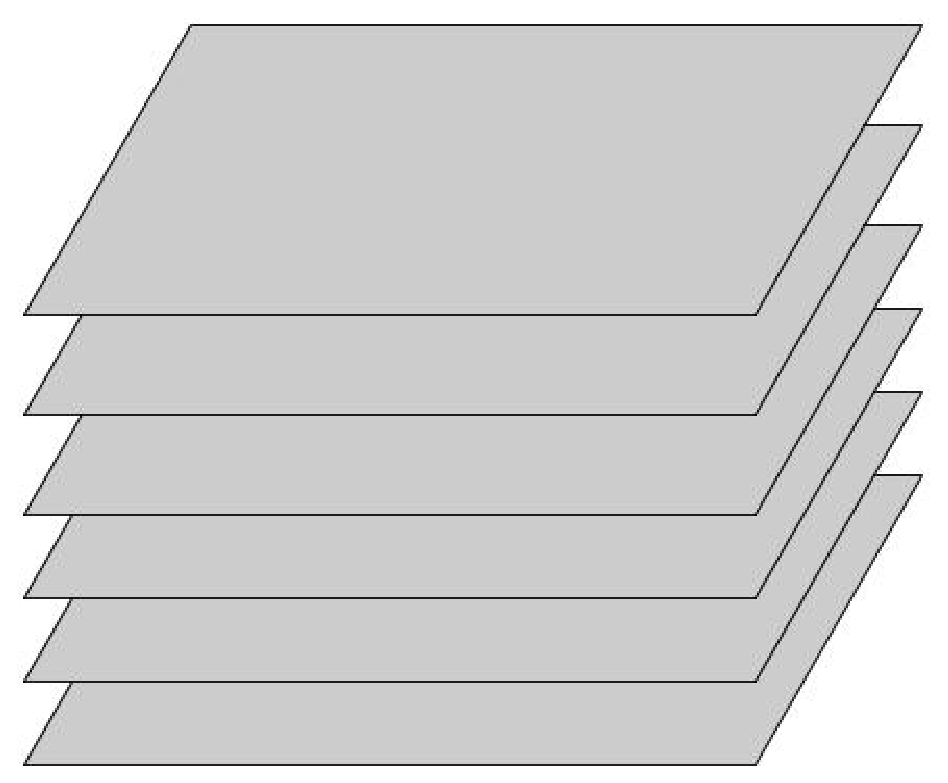
\includegraphics[width=\textwidth]{Images/slices-vertical.eps}
  \caption{Vertical slices}\label{fig:3tensor-verticalslices}
 \end{subfigure}
\caption{3rd-order tensor slices}\label{fig:3tensor-slices}
\end{figure}

The \textit{norm} of a tensor $\mathcal{X}\in \mathbb{R}^{I_1\times I_2 \ldots \times I_N}$ is analogous to the matrix Frobenius norm, i.e.
\begin{equation}
||\mathcal{X}|| = \sqrt{\sum_{i_1=1}^{I_1}\sum_{i_2=1}^{I_2}\cdots\sum_{i_N=1}^{I_N} x_{i_1i_2\ldots i_N}^2 } 
\end{equation}\label{eq:Frobenius-norm}

%also include here
%inner product of two same-size tensors

% rank one tensors
$\mathcal{X}$ is a \textit{Rank-one} tensor if it is equal to the outer product of N vectors, i.e.,
\[
\mathcal{X} = a^{(1)}\otimes a^{(2)} \otimes \ldots \otimes a^{(N)}
\]

% simetry

% diagonal tensor

\subsubsection{Unfolding and Folding Tensors}

\textit{Unfolding} is the process of \textit{matricization} of a tensor. In other words, elements of a tensors are sorted to assemble a matrix. The mode-$k$ unfolding of a tensor $\mathcal{X}\in \mathbb{R}^{I_1\times I_2 \ldots \times I_N}$ is denoted by  $X_{(k)} \in \mathbb{R}^{I_1\times \prod_{k'\neq k}I_{k'} }$ and arrenges the mode-$k$ tensor fibers as columns of resulting matrix. In addition, Kolda \cite{Kolda2009} presents a more general procedures of unfolding

% figure mode-k unfolding and folding

% \subsubsection{Tensor products}

% \paragraph{Mode-k product}

% \paragraph{Kronecker product}

% \paragraph{Khati-Rao product}

% \paragraph{Hadamar product}

% \paragraph{Outer product}


Ding and Wei \cite{Ding2015} present a fast algorithm for Hankel tensor-vector products. And \cite{Dourbal2016} a method of fast linear transform algorithm synthesis for an arbitrary tensor.

\section{Tensor Decomposition}

% The tensor decomposition problem consists of break down a tensor in a 

Tensor decomposition originated with Hitchcock in 1927 \cite{Hitchcock1927}, and the the multi-way model is attribuited to Cattell in 1944 \cite{Cattell1944}.

Tensor works had attention in 60s with Tucker (\cite{Tucker1963}, \cite{Tucker1964}, \cite{Tucker1966}) and Carroll and Chang \cite{Carroll1970} and Harshman in 1970 \cite{Harshman1970} with applications in psychometrics. In 1981 Appellof and Davidson \cite{Appellof1981} used tensor decomposition in chemometrics which have been an popular field of application of tensor decomposition since then.

As shown figure \ref{fig:applications}, in last twenty years tensor decomposition applications have expanded to many fields such as signal processing, numberical linear algebra, computer vision, numerical analysis, neuroscience, data mining, graph analysis. Figure \ref{fig:applications} shows seminal papers which opened broad application fields to tensor decomposition, plot also shows the amount of documents published about these works according to Scopus.

\begin{figure}[!ht]
\centering
 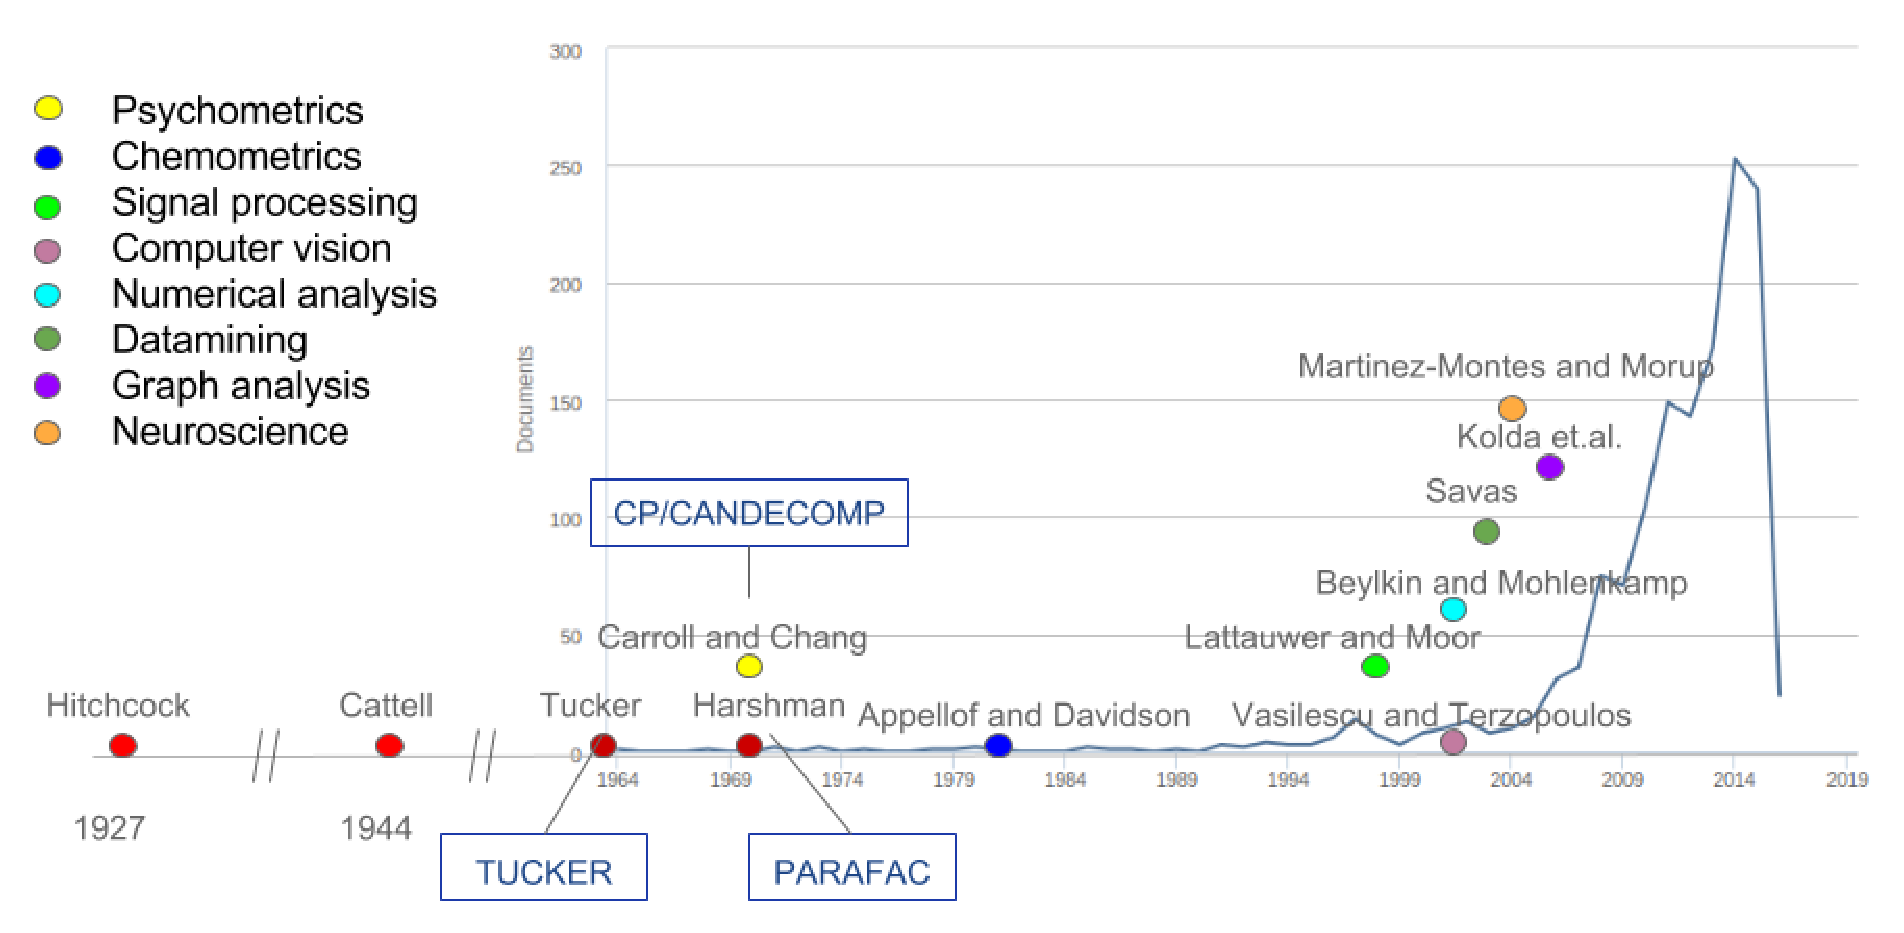
\includegraphics[scale=0.5]{Images/time-line.eps}
 \caption{Time-line of tensor decomposition}\label{fig:applications}
\end{figure}

% \begin{figure}[!ht]
% \centering
%  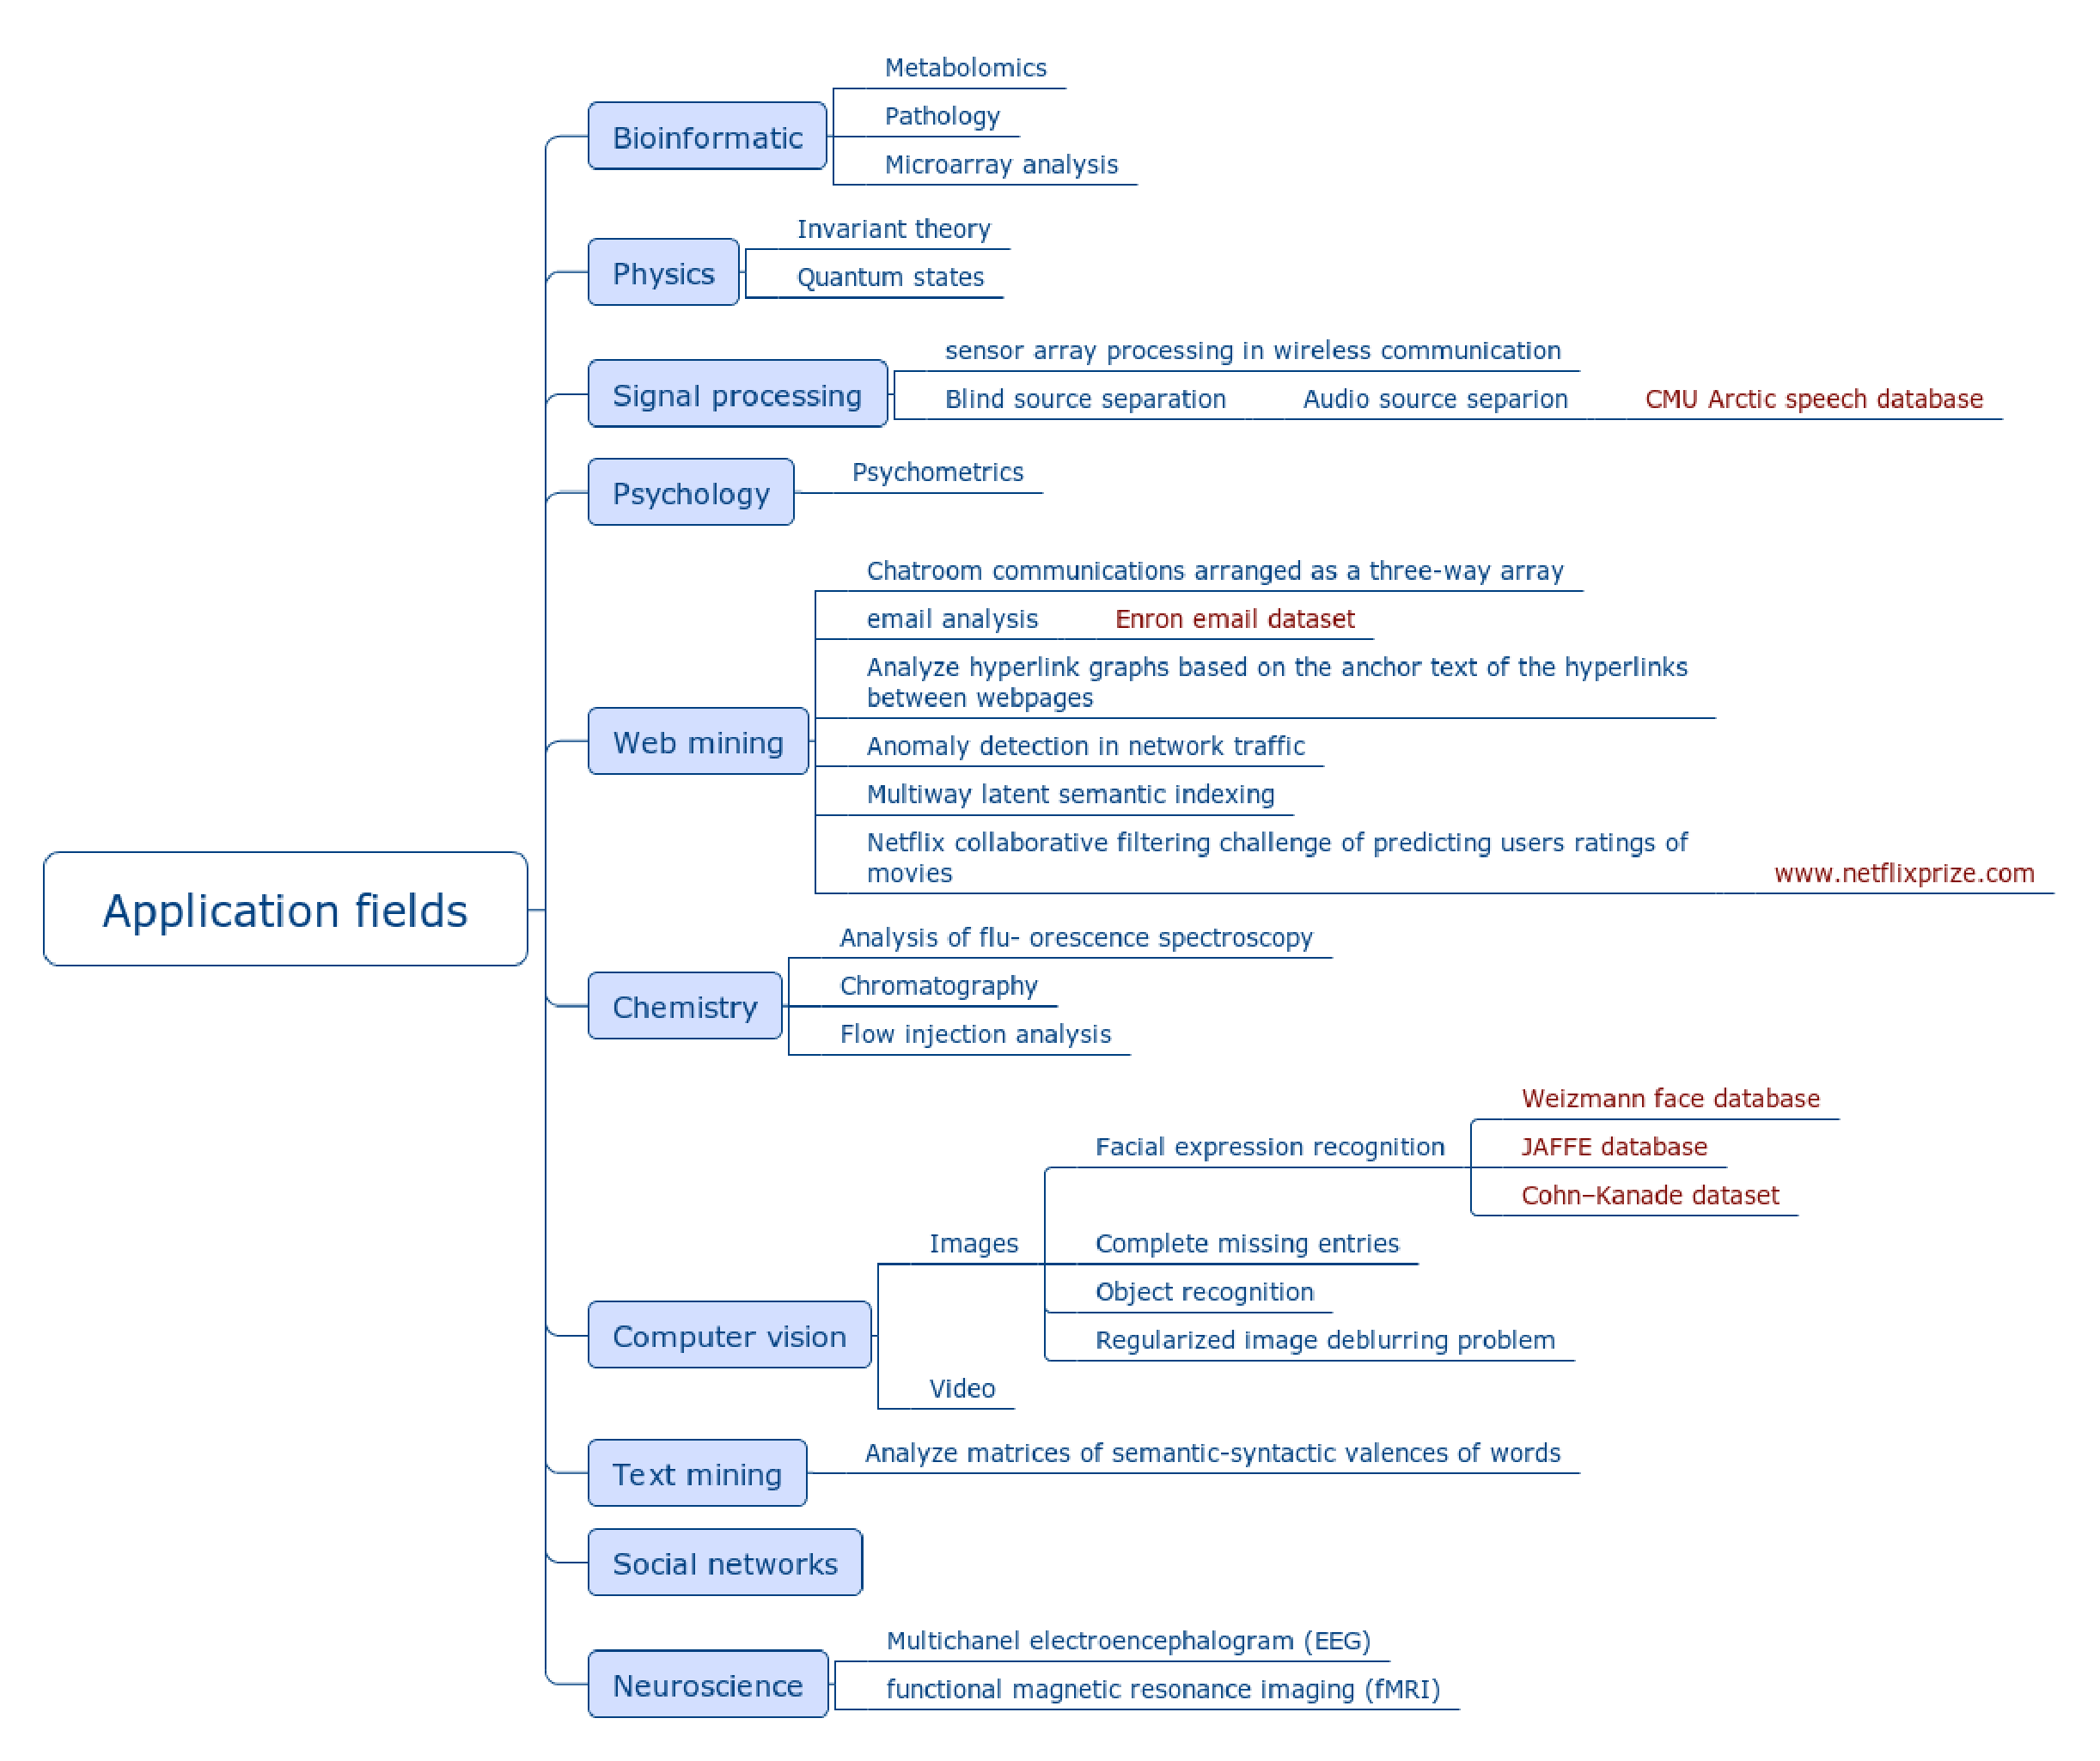
\includegraphics[scale=0.3]{Images/application_fields.eps}
%  \caption{Application fields of tensor decomposition}\label{fig:applications}
% \end{figure}


% Extend applications descriptions and cite paper and survey Specific for each field.

Kolda \cite{Kolda2009}, Acar \cite{Acar2009} and \cite{Comon2014} present an exhaustive and detailed review of fundamental decomposition methods and applications. Furthermore, \cite{Dartois2016} presents tensor properties as extension of estructural properties of matrices. On the other hand, Fanaee and Gama \cite{Fanaee-T2016} introduce an interdisciplinary survey about tensor-based anomaly detection.

In following sections we explain some of basic methods to tensor decomposition which have been inspiration to many others methods propossed. Also, we summarize recently  works and approaches of tensor decomposition on different application fields.

%extend and compare
\paragraph{Chemometrics}

\cite{Chaudhury2014} Propose a computationally efficient technique for the solution of multi-dimensional PBMs of granulation via tensor decomposition

%bioinformatics
\paragraph{Bioinformatics}

In \cite{Acar2015} and \cite{Acar2014} a multimodal problem is addressed, the authors formulate data fusion as a coupled matrix and tensor factorization problem and discuss its extension to a structure-revealing data fusion model in metabolomics.


\paragraph{Image processing}

\cite{An2015} NNTF for facial expression recognition


\paragraph{Machine Learning}

\cite{Anandkumar2012} Tensor decompositions for learning latent variable models

\paragraph{Text mining}

\cite{Anisimov2014} This paper describes a method for automatic detection of semantic relations between concept nodes of a networked ontological knowledge base by analyzing matrices of semantic-syntactic valences of words. These matrices are obtained by means of nonnegative factorization of tensors of syntactic compatibility of words. 


\paragraph{Numerical analysis}
 
\cite{Antolin2015} use of the sum-factorization for the calculation of the integrals arising in Galerkin isogeometric analysis. While introducing very little change in an isogeometric code based on element-by-element quadrature and assembling, the sum-factorization approach, taking advantage of the tensor-product structure of splines or NURBS shape functions, significantly reduces the quadrature computational cost.

\cite{Benner2016} Fast iterative solution of the Bethe-Salpeter eigenvalue problem using low-rank and QTT tensor approximation.


\cite{Cherif2008} Blind identification of a second order Volterra-Hammerstein series using cumulant cubic tensor analysis.

\paragraph{Neuroscience}

\cite{Arnedo2015} Decomposition of brain diffusion imaging data uncovers latent schizophrenias with distinct patterns of white matter anisotropy, using NNTF to clustering.


\paragraph{Signal processing}

Cichocki et.al. \cite{Cichocki2015} sum up tensor decomposition approaches for signal processing problems.

Barker and Virtanen \cite{Barker2014} deal with monaural sound source separation problem using NNTF of modulation spectrograms.

\cite{Bilen2016} Necessity to manually assign the NTF components to audio sources in order to be able to enforce prior information on the sources during the estimation process, Automatic Allocation of NTF Components for User-Guided Audio Source Separation

\cite{Fitzgerald2006} propose a shifted 2D non-negative tensor factorisation algorithm which extends non-negative matrix factor 2D deconvolution to the multi-channel case. The use of this algorithm for multi-channel sound source separation of pitched instruments is demonstrated.

\paragraph{Other applications}

\cite{Espin-Noboa2016} Discovering and Characterizing Mobility Patterns in Urban Spaces: A Study of Manhattan Taxi Data. by using non-negative tensor factorization (NTF), we are able to cluster human behavior based on spatio-temporal dimensions. Second, for understanding these clusters, we propose to use HypTrails, a Bayesian approach for expressing and comparing hypotheses about human trails.

\cite{Figueiredo2014} NTF factorization for household electrical seasonal consumption disaggregation


\subsection{Tensor Factorization Methods}


\begin{figure}[!ht]
\centering
 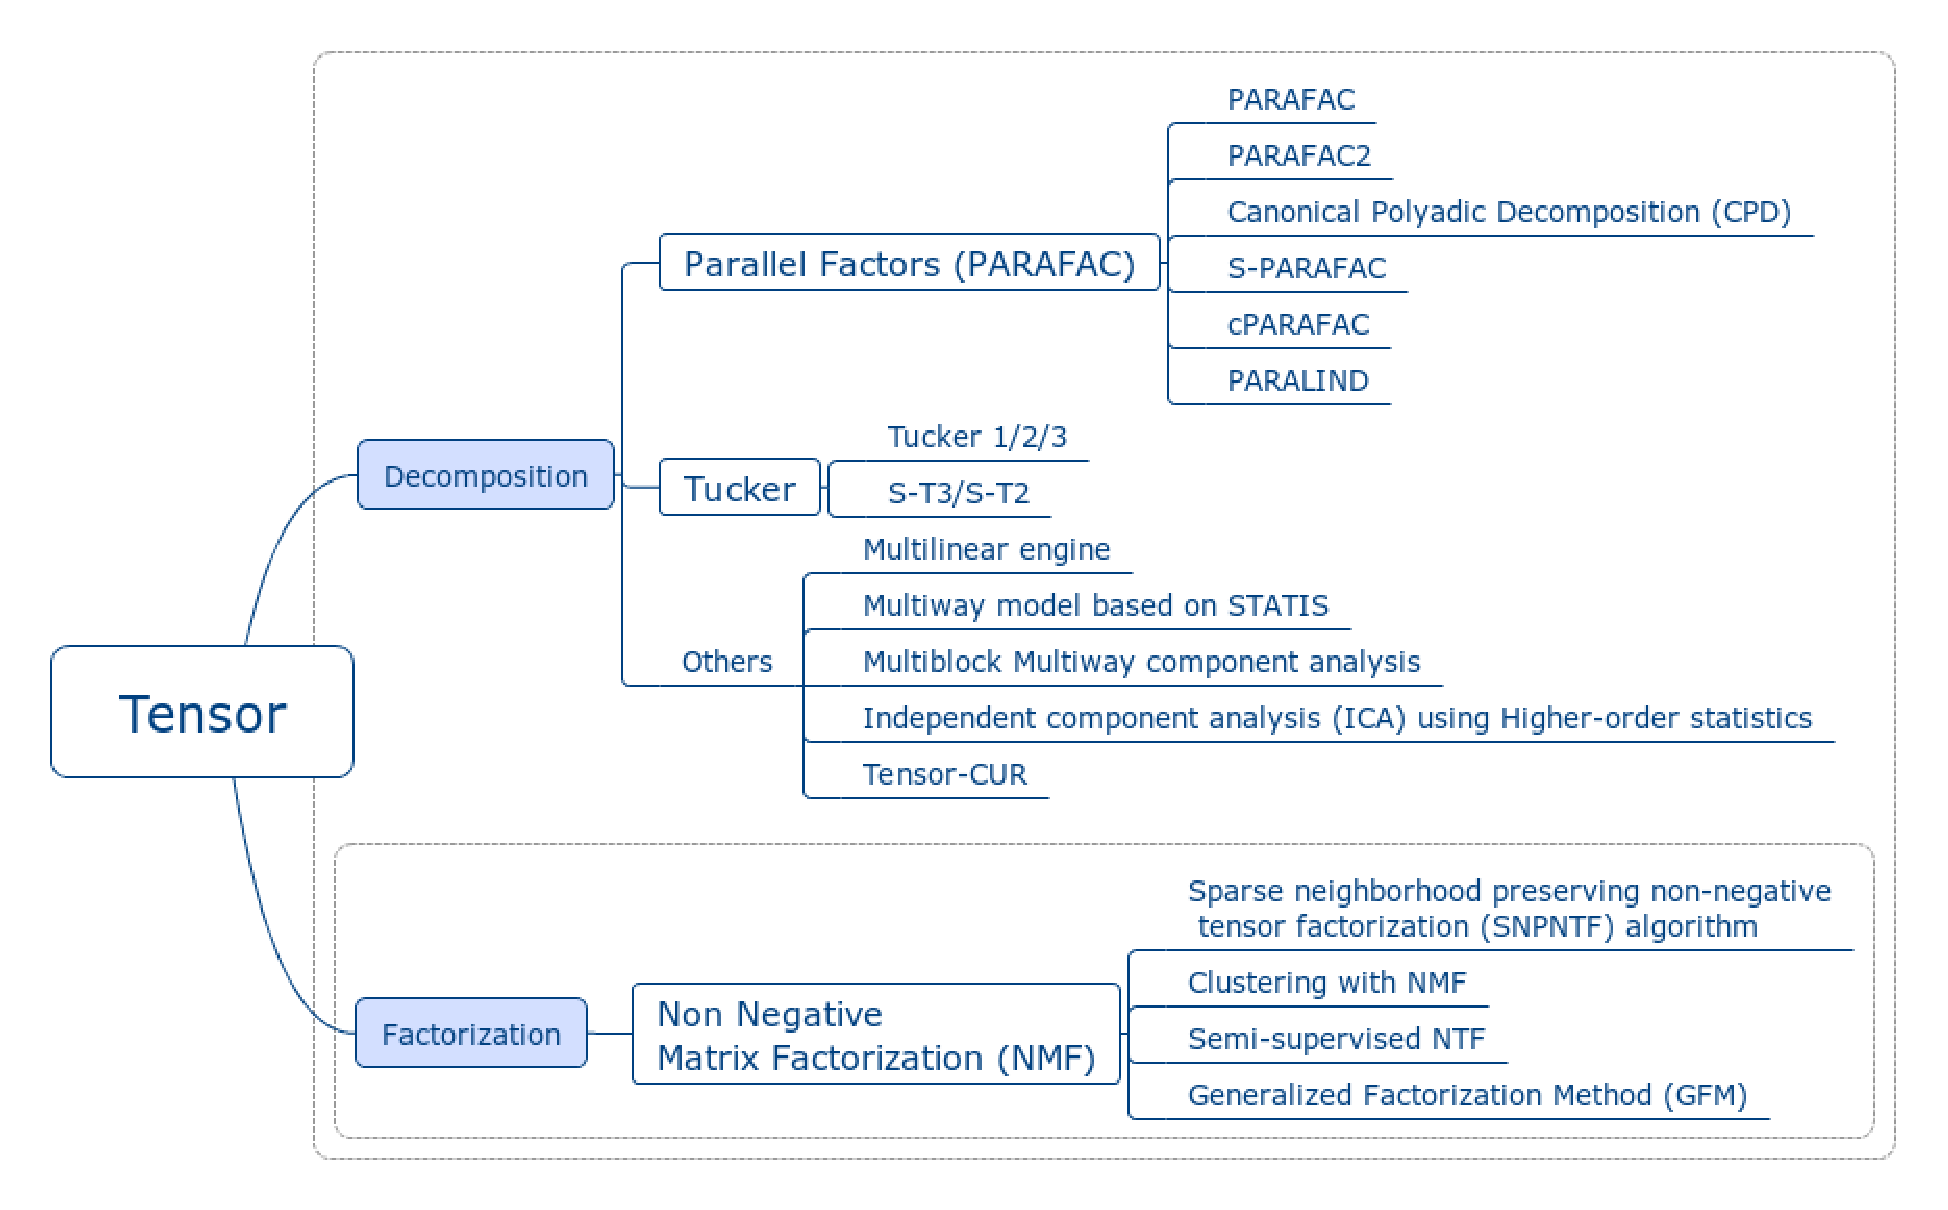
\includegraphics[scale=0.5]{Images/tensor_decomposition_methods.eps}\label{fig:methods}
 \caption{Tensor decomposition methods}
\end{figure}

\subsubsection{Canonica Polyadic Decomposition / PARAFAC}

%check missed cite
Canonica Polyadic (CP) decomposition (\cite{Kolda2009}, \cite{Mocks1988}), CANDECOMP \cite{Carroll1970} or PARAFAC \cite{Harshman1970} decompose a tensor as a finite sum of rank-one tensors. For instance, given a third order tensor $\mathcal{X}\in\mathbb{R}^{I\times J\times K}$, CP decomposition express it as 

\begin{equation}
 \mathcal{X}\approx \sum_{r=1}^{R}a_r\otimes b_r \otimes c_r
\end{equation}\label{eq:cp}

where $a_r\in\mathbb{R}^I$, $b_r\in\mathbb{R}^J$, $c_r\in\mathbb{R}^K$ and $R$ is a positive integer.


%figure

Domanov \cite{Domanov2015} shows relaxed uniqueness conditions and algebraic algorithm for Canonical polyadic decomposition, as well as a reduction to generalized eigenvalue decomposition \cite{Domanov2014} and uniqueness properties \cite{Domanov2013} of third-order tensors.


\subsubsection{TUCKER Decomposition}

%check missing cites
Tucker decomposition was introduced by Tucker (\cite{Tucker1963}, \cite{Tucker1964}). It is also named N-mode PCA \cite{Kapteyn1986}, High-order SVD (HOSVD) \cite{DeLathauwer2000} or N-mode SVD \cite{Vasilescu2002}.

The Tucker decomposition is a form of higher-order PCA \cite{Kolda2009}. It descomposes a tensor into a core tensor $\mathcal{G}$ multiplied by a matrix algong each mode. For instance, given a third order tensor $\mathcal{X}\in\mathbb{R}^{I\times J\times K}$, Tucker decomposition express it as 

\begin{equation}
 \mathcal{X}\approx \mathcal{G}\times_1 A \times_2 B \times_3 C
\end{equation}

Where $\times_k$ is the mode-$k$ product, $A\in \mathbb{R}^{I\times P}$, $B\in \mathbb{R}^{J\times Q}$, $C\in \mathbb{R}^{K\times R}$ are the factor matrices (usually orthogonals) and can be interpreted as the principal components for each mode. $\mathcal{G}\in\mathbb{R}^{P\times Q \times R}$ is the core tensor and its entries show the interactions between the different components.

\subsubsection{Non-negative Tensor Factorization}

\paragraph{Non-negative Matrix Factorization}

The general problem of non-negative matrix factorization (NMF) is to decompose a matrix $X \in \mathbb{R}_{\geq 0}^{n\times l}$ into two matrix factors: basis $W \in \mathbb{R}_{\geq 0}^{n\times k}$  and coefficients $H \in \mathbb{R}_{\geq 0}^{k\times l}$, i,e.

\begin{equation}
X\cong W H\label{eq:matrix-factorization}
\end{equation}
 
The factorization problem can be seem as an optimization problem:

\begin{equation}
\min_{W,H}d(X,WH)\label{eq:objective-function-factorization}
\end{equation}


where $d(,)$ is a distance or divergence function and the problem could have different types of restrictions. For instance, if $d(,)$
is the Euclidean Distance and there are not restrictions, the problem is solved by finding the SVD; if $X$, $W$ and $H$ are restricted
to be positive, then the problem is solved by NMF. An comprehensive survey of NMF variants and algorithms is finded in \cite{Wang2013}.
%check missing reference
One NMF approach is Symmetric-NMF \cite{Ding2005}, (SNMF) which produces a factorization: 

\begin{equation}
(X_{lxn}^{T}X_{nxl})=H_{lxk}H_{kxl}^{T}\label{eq:symmetric-nmf}
\end{equation}

An important characteristic of this version of NMF is that it is amenable to be used as a kernel method. This is discussed in the next subsection.

\paragraph{Non-negative Tensor Factorization}%rewrite and chec since this section is a direct copy&paste from (Wang and Zhang, 2013)


An natural extension of nonnegative matrix factorization with high-order arrays is nonnegative n-dimensional tensor factorization (n-NTF). This kind of generalization is indeed not trivial since NTF possesses many new properties varying from NMF (\cite{Hazan2005}, \cite{Morup2008}).  

% (cp Wang and Zhang, 2013) 
First, the data to be processed in NMF are vectors in essence. However, in some applications the original data may not be vectors, and the vectorization might result in some undesirable problems. For instance, the vectorization of image data, which is two dimensional, will lose the local spatial and structural information. Second, one of the core concerns in NMF is the uniqueness issue, and to remedy the ill-posedness some strong constraints have to be imposed. Nevertheless, tensor factorization will be unique under only some weak conditions. Besides, the uniqueness of the solution will be enhanced as the tensor order increases\cite{Wang2013}.

%check miss cite
There are generally two types of NTF model—NTD \cite{Morup2008} and more restricted NPARAFAC \cite{Hazan2005}, whose main difference lies in the core factor tensor. As for the solution, there are some feasible approaches. For example, NTF can be restated as regular NMF by matricizing the array \cite{Welling2001}, \cite{Morup2008}. Or the alternating iteration method can be utilized directly on the outer product definition of tensors \cite{Hazan2005}, \cite{Shashua2005}, \cite{Benetos2010}. Similarly, SED, GKLD and other forms of divergence can also be used as the objective functions \cite{Benetos2010}, \cite{Cichocki2007}, \cite{Zafeiriou2011}. And some specific update models can adopt the existing conclusions in NMF. %For thorough understanding one may refer to [9], [122]. 
%What must be scrutinized here is that the convergence of these algorithms is not guaranteed by the simple generation from matrix to tensor forms in itself.

%What’s more, the concepts in Constrained NMF can also be incorporated in NTF, such as sparse NTF [123], [124], [125], discriminant NTF [126], NTF on manifold [127], and the like.


%Include Cichocki approaches

\subsubsection{Other methods}

 The tensor decomposition addressed in \cite{Bernardi2013} may be seen as a generalization of Singular Value Decomposition of matrices. They consider general multilinear and multihomogeneous tensors. Then, they show how to reduce the problem to a truncated moment matrix problem and give a new criterion for flat extension of Quasi-Hankel matrices. 

 
\subsection{Kernel methods}

In contrast with traditional learning techniques, kernel methods do not need a vectorial representation of data. Instead, they use a kernel function. Therefore, kernel methods are naturally applied to unstructured, or complex structured, data such as texts, strings, trees and images \cite{Shawe-Taylor2004}. 

Informally, a kernel function measures the similarity of two objects. Formally, a kernel function, $k:X\times X\rightarrow\mathbb{R}$,
maps pairs $(x,y)$ of objects in a set $X$, the problem space, to the reals. A kernel function implicitly generates a map, $\Phi:X\rightarrow F$, where $F$ corresponds to a Hilbert space called the feature space. The dot product in $F$ is calculated by $k$, specifically $k(x,y)=<\Phi(x),\Phi(y)>_{F}$. Given an appropriate kernel function, complex patterns in the problem space may correspond to simpler patterns in the feature space. For instance, non-linear patterns in the problem space may correspond to linear patterns in the feature space. 


Both $k$-means and SNMF have kernelized versions, which receive as input a kernel matrix instead of a set of sample represented by feature vectors. The kernel version of $k$-means is called, unsurprisingly, kernel $k$-means (KKM). In the case of SNMF, the kernelized version works as follows.

SNMF starts with an initial estimation of the matrix factor $H$ and iteratively update it using the updating equation:

\[
H_{i,k}=H_{i,k}(1-\beta+\beta\frac{((X^{T}X)H)_{i,k}}{(HH^{T}H)_{i,k}})
\]


The kernel version of the algorithm is obtained by using a kernel matrix $K$ instead of the expression $(X^{T}X)$, where $K$ is an
$l\times l$ matrix with $K_{i,j}=k(x_{i},x_{j}).$ There are different types of kernels some of them general and some of them specifically defined for different types of data. The most popular general kernels are the linear kernel 

\begin{equation}
k(x,y)=<x,y>,\label{eq:id-kernel}
\end{equation}

 the polynomial kernel 
 
\[
k(x,y)=p(<x,y>),
\]

 where $p(\,)$ is a polynomial with positive coefficients, and the Gaussian (or RBF) kernel 
 
\begin{equation}
k(x,y)=e^{\frac{\left\Vert x-y\right\Vert ^{2}}{2\sigma^{2}}}.\label{eq:Gaussian-kernel}
\end{equation}


The cluster centroids estimated by the kernel versions of both algorithms are in the feature space and correspond to the points $C_{j}=\frac{1}{n}\sum_{x_{i}\in C_{j}}\Phi(x_{i})$. However, we are interested on the pre-image in the original space of this centroids, i.e., points $\hat{C}_{j}$ such that $\Phi(\hat{C}_{j})=C_{j}$. However, it is possible that a exact pre-image may not even exist, so we look for the $\hat{C}_{j}$ that minimizes the following objective function:$\min_{\hat{C}_{j}}\left\Vert \hat{C}_{j}-C_{j}\right\Vert ^{2}$. According to Kwok et al. \cite{kwok2004preimage}, the optimum $C_{j}$ can be found by iterating the following fixed-point formula:

\begin{equation}
\hat{C}_{j}^{t+1}=\frac{\sum_{i=1}^{N}\exp(\frac{-||\hat{C}_{j}^{t}-x_{i}||)}{s})x_{i}}{\sum_{i=1}^{N}\exp(\frac{-||\hat{C}_{j}^{t}-x_{i}||}{s})}\label{eq:back-projection}
\end{equation}


\section{Kernel Non-negative Matrix Factorization}

Kernel Non-negative Matrix Factorization (KNMF) can be naturally derivated of convex NMF (\cite{Kulis2006}, \cite{Li2005} and \cite{Rosipal2001}). Given a kernel function $\phi:x\in X \rightarrow \phi(x)\in F $, mapping for $N$ elements $\phi(X) = [ \phi(x_1),\ldots \phi(x_N) ]$. Then, KNMF can be defined as
\begin{equation}
 \phi(X)\cong\phi(X)WH^T
\end{equation}\label{eq:KNMF}

Therefore, the cost function to minimize is

\begin{equation}
 || \phi(X) - \phi(X)WH^T ||_F^2 = tr(K) - 2 tr(H^TKW)+tr(W^TKWH^TH)
\end{equation}

 Where kernel $K=\phi^T(X)phi(X)$
 
 

\subsection{General problems}

%  Usually, tensor factorization address the folowing problems independent of the application: blind source separation, tensor completion.

 \subsection{Blind Source Separation}
 
 %rewrite, it is c&p
Blind source separation (BSS) and related methods, e.g., independent component analysis (ICA), employ a wide class of unsupervised learning algorithms and have found important applications across several areas from engineering to neuroscience \ref{Cichocki2009}. The recent trends in blind source separation and generalized (flexible) component analysis (GCA) are to consider problems in the framework of matrix factorization or more general multi-dimensional data or signal decomposition with probabilistic generative models and exploit a priori knowledge about true nature, morphology or structure of latent (hidden) variables or sources such as nonnegativity, sparseness, spatiotemporal decorrelation, statistical independence, smoothness or lowest possible complexity. The goal of BSS can be considered as estimation of true physical sources and parameters of a mixing system, while the objective of GCA is to find a reduced or hierarchical and structured component representation for the observed (sensor) data that can be interpreted as physically or physiologically meaningful coding or blind signal decomposition. The key issue is to find such a transformation or coding which has true physical meaning and interpretation.

 \subsection{Tensor completion}
 
 In tensor completion, an given incomplete tensor is given, i.e. some of its entries are missing and we should complete that. Following Ji Lu et.al \cite{Liu2013} notation,  low rank matrix completion is noted as

\begin{equation} 
 \begin{split}
  \min_X & \text{ rank}(X)\\
  \text{s.t. } & X_\Omega = M_\Omega
 \end{split}
\end{equation}

where $\Omega$ is an index set, then $X_\Omega$ is coping entries of $X$ in the indexes $\Omega$ and missed entries $\hat{\Omega}$ would be $0$

The missing entries in $X$ are determined in order to minimize the matrix $X$ rank. i.e. a non convex optimization problem since rank is nonconvex.

Frequently, trace norm (or nuclear norm) $||\cdot ||_*$ is used to approximate the rank of matrices.

Trace norm is the tighest convex envelop for the matrices rank.

\begin{equation} 
 \begin{split}
  \min_X & ||X||_*\\
  \text{s.t. } & X_\Omega = M_\Omega
 \end{split}
\end{equation}

Since tensor is a generalization of the matrix concept, we generalize the  optimization problem as

\begin{equation} 
 \begin{split}
  \min_{\mathcal{X}} & ||\mathcal{X}||_*\\
  \text{s.t. } & \mathcal{X}_\Omega = \mathcal{T}_\Omega
 \end{split}
\end{equation}

Where $\mathcal{X}$ and $\mathcal{T}$ are $n$-order tensors with identical size.

Acar et.al \cite{Acar2011} presents a scalable tensor factorization method to deal with completion problem using PARAFAC method. Cao \cite{Cao2015} propose a new tensor completion model via folded-concave penalty for estimating missing values in tensor data.To solve the resulting nonconvex optimization problem, we develop a local linear approximation augmented Lagrange multiplier (LLA-ALM) algorithm which combines a two-step LLA strategy to search a local optimum of the proposed model efficiently. They show numerical results in image and video data sets and compare with nuclear norm penalization method in order of demostrate its advantage in terms of the accuracy and robustness.


Chen \cite{Chen2014} propose a method to deal with the completion problem when the number of missing entries increases, since factorization schemes may overfit the model because of incorrectly predefined ranks, while completion schemes may fail to interpret the model factors.  
Hence, they present an approach to complete the missing entries and simultaneously capture the underlying model structure that combines a rank minimization technique with Tucker model decomposition. Moreover, as the model structure is implicitly included in the Tucker model, they  use factor priors, which are usually known a priori in real-world tensor objects, to characterize the underlying joint-manifold drawn from the model factors.



% \subsection{Tensor probability}

% Given a sample set

\section{Problem Statement}

%Importance of tensor decomposition
%	- Advantage over matrix factorization
%Why use kernels
%Challenges of kernelized methods
%Literature gap regard to kernel tensor decomposition

Tensor factorization (including matrix factorization) is central to different important tasks in machine learning and information retrieval such as: clustering, latent topic analysis, recommendation, blind source separation, completion, denoising, among others. 

The widespread use of multisensor technology and the emergence of big data sets have highlighted the limitations of standard flat-view matrix models and the necessity to move toward more versatile data analysis tools \cite{Cichocki2015}. Conventional methods preprocess multiway data by arranging them into a matrix, which might lose the original multiway structure of the data  \cite{Wang2013}. Hence, tensors address multimodal or multiview data, and tensor factorization brings tools to perform common machine learning tasks.%move this paragraph to the justification

%highlight problem
%problem dimensionality tensor and kernel trick to deal with it
%exploit no-linear relations

Tensor factorizations have several advantages over two-way matrix factorizations including uniqueness of the optimal solution and component identification even when most of the data is missing  \cite{Morup2011}.

On the other hand, kernel methods are ubiquitous in machine learning, performance of these methods have been broadly demostrated, and there are evidence between some types of kernels and robustness. However, there are few exploration of kernel tensor factorization approaches.

A satisfactory solution of this general challenge requires to answer some particular\textbf{research question}: 

\begin{itemize}
 \item How incorporate kernel methods in tensor factorization in order to deal with multiway data? %- exploratory
\end{itemize}

An answer to the question derivate in a method which factorize a given tensor in the feature space induced by a Kernel function. Naturally, to inquire about the effects of decompose tensors in an space induced by a kernel function open space to evaluate the proposal method performance as well as its capabilities dealing with multimodal data, scalability and robustness to noise and outliers.


%  \item \textbf{GENERAL AND SPECIFIC OBJECTIVES} 
% 7. OBJETIVO GENERAL Y OBJETIVOS ESPECÍFICOS: (Evaluables)


\section{Goals}

% The general problem addressed by this research proposal is the design of non-supervised learning algorithms, in particular tensor factorization algorithms, applied in the space induced by a kernel function. 

 \subsection*{General objective}

To design, implement and evaluate a kernel-based tensor factorization algorithm for unsupervised learning.
 
\subsection*{Specific objectives}

\begin{itemize}
\item To evaluate different strategies for combining kernel-based methods with matrix and tensor factorization techniques.
\item To design an algorithm for kernel-based tensor factorization.
\item To develop an efficient implementation of the algorithm able to deal with large scale data sets.
\item To assess the effectivity of the method in specific unsupervised learning tasks.
\end{itemize}


\section{Jusification}


Due to the rich characteristics of natural processes and environments, it is rare that a single acquisition method provides complete understanding thereof. Information about a phenomenon or a system of interest can be obtained from different types of instruments, measurement techniques, experimental setups, and other types of sources. The increasing availability of multiple data sets that contain information, obtained using different acquisition methods, about the same system, introduces new degrees of freedom that raise questions beyond those related to analyzing each data set separately.

By treating that natural high-order array as a matrix, information is lost since lack the original multiway structure of the data.


Tensor factorizations have several advantages over two-way matrix factorizations including uniqueness of the optimal solution and component identification even when most of the data is missing \cite{Morup2011}. 

multiway decomposition techniques explicitly exploit the multiway structure that is lost when collapsing some of the modes of the tensor in order to analyze the data by regular matrix factorization approaches.

Tensor decompositions are in frequent use today in a variety of fields ranging from psychology, chemometrics, signal processing, bioinformatics, neuroscience, web mining, and computer vision to mention but a few.

Matrix and analogous tensor factorization is central to different important tasks in machine learning and information retrieval such as: clustering, latent topic analysis, recommendation, tensor completion, blind source separation, among others.



\section{Methodology}
% \item \textbf{METHODOLOGY}\\ 
% % 8. METODOLOGÍA: (Descripción del procedimiento a emplear para obtener los 
% objetivos propuestos).
% % 


This research is an experimental study with experimental design and quantitative strategies such as accuracy, specificity and sensitivity in a cross-sectional study with standard images.

Each specific objective is to be attained through the following approaches:

\begin{enumerate}[(a)]
 \item \textit{Review kernel-based methods proposed to matrix and tensor factorization}. A systematic literature review will be leaded to identify the matrix and tensor factorization methods witch incorporate kernels. Methods to address the pre-image problem in kernel-methods also will be included in this review.

\item \textit{Design and implementation of Kernel Tensor Factorization algorithm}. An kernel matrix factorization methods will be adapted to use tensorial kernels. Efficient implementations will be developed exploiting particularities of the used kernels. 
\item \textit{Strategy to assess method precision in specific unsupervised-learning tasks}. In order to evaluete algorithm effectivity solving completion and blind source separation problems, the method will be applied in both synthetic and real world datasets to assess performance.

%to deal with noise and outliers, a collection of synthetic and real datasets with different degrees of contamination will be assembled. An experimental setup for algorithm evaluation will be designed taking into account different factors (kernel type, contamination degree, etc) and the robustness measures as influence curve and/or the breakdown bound adapted to tensor factorization.

\item \textit{Measuring algorithm scalability}. An theoretical time and space complexity bound will be assesed to the algorithm. Furthermore, an parallelizable version of algorithm will be suggested.
\end{enumerate}


%\subsection{Data}
%datasets

% % 9. ACTIVIDADES A DESARROLLAR:
 
\section{Activities}

Project activities and results are structured within \textit{Work Packages} (WP) in terms of \textit{Tasks} (T) and \textit{Deliverables}, as described below.

\subsection*{WP0: Cross activities - Divulgation}
\subsubsection*{TASKS }
\begin{itemize}
\item T0: Proposal writing.
\item T1: Proposal presentation.
\item T2: Write articles for journals or conferences.
\item T3: Dissertation writing.
\item T4: Dissartation defence.
\end{itemize}
\subsubsection*{DELIVERABLES }
\begin{itemize}
 \item Proposal
 \item Articles
 \item Dissertation
\end{itemize}



\subsection*{WP1: Literature Review}
An systematic literature review will be done to review tensor factorization methods, in particular, 
kernel-based matrix and tensor factorization methods. Furthermore, we will include methods to address the pre-image problem in kernel methods.
\subsubsection*{TASKS }
\begin{itemize}
\item T0: Stablish research question and criteria for document inclusion.
\item T1: Search process
\item T2: Quality assessment and data collection
\item T3: Data analysis
\end{itemize}
\subsubsection*{DELIVERABLES }
\begin{itemize}
\item Document summarizing literature review
\end{itemize}

\subsection*{WP2: Evaluation of strategies for combining kernel-based methods with matrix and tensor factorization techniques}
According to literature review, we will analyze and contrast strategies for combining kernel-based methods with matrix and tensor factorization techniques
\subsubsection*{TASKS}
\begin{itemize}
\item T0: Review and compare methods
\end{itemize}
\subsubsection*{DELIVERABLES}
\begin{itemize}
\item Technical report 
\end{itemize}

\subsection*{WP3: Design of algorithm for kernel-based tensor factorization.}
\subsubsection*{TASKS}
\begin{itemize}
\item T0: Model tensor factorization algorithm.
\item T1: Address pre-image problem if it is pertinent.
\item T2: Stablish how to apply the algorithm to tensor completion problem and blind source separation.
\end{itemize}
\subsubsection*{DELIVERABLES}
\begin{itemize}
 \item Algorithm pseudocode
\end{itemize}


\subsection*{WP4: Developing an efficient algorithm implementation able to deal with large scale data sets.}
\subsubsection*{TASKS}
\begin{itemize}
\item T0: Adapt algorithm to scale if it is required.
\item T1: Implement kernel tensor factorization algorithm.
\item T2: Design experimental setup.
\item T3: Execute experiments and measure performance.
\item T4: Collect and analyze results
\end{itemize}
\subsubsection*{DELIVERABLES}
\begin{itemize}
 \item source code
 \item Technical report
\end{itemize}



\subsection*{WP5: Assessing the effectivity of the method in specific unsupervised learning tasks.}
\subsubsection*{TASKS}
\begin{itemize}
\item T0: Design experimental setup.
\item T1: Execute experiments and measure performance.
\item T2: Collect and analyze results
\end{itemize}
\subsubsection*{DELIVERABLES}
\begin{itemize}
 \item source code
 \item Technical report
\end{itemize}
% 
% 
% Project activities and results are structured within \textit{Work Packages} 
% (WP) in terms of \textit{Tasks} and \textit{Deliverables}, as described below.
% 
% \subsection*{WP0: PROPOSSAL}
% 
% This WP will assure a suitable scope of propossal due to evaluation of risk 
% and feasibility. In addition, activities and schedule will be delimited in 
% concordance with objectives stablished.
% 
% \subsubsection*{TASKS}
% \begin{itemize}
%  \item T0.1: Propossal review
%  \item T0.2: Literature review.
% \end{itemize}
% 
% 
% \subsubsection*{DELIVERABLES}
% \begin{itemize}
%  \item D0.1: A survey paper reporting the literature review.
%  \item D0.2: Final propossal
% \end{itemize}
% 
% 
% \subsection*{WP1: MANAGEMENT }
% 
% This WP will ensure effective planning, implementation, coordination and achievement of the project activities, including successful completion of the tasks and timely production of deliverables.
% 
% \subsubsection*{TASKS }
% \begin{itemize}
% \item T1.1: ADMINISTRATION AND MANAGEMENT. Will take care of financial and resource accounting. It will also be in charge of managing the relations with collaborating institutions and administrative bodies within.
% \item T1.2: PROJECT FOLLOW UP AND QUALITY CONTROL. Will act as the final stage before delivery hand over to ensure compliance and coherence. Also, it will follow up project progress anticipating corrective actions and assessing risk mitigation actions.
% \end{itemize}
% 
% \subsubsection*{DELIVERABLES}
% \begin{itemize}
% \item D1.1: Periodic technical project reports.
% % \item D1.2: Periodic financial project reports
% \end{itemize}
% 
% \subsection*{WP2: MEASURING ROBUSTNESS}
% 
% 
% \subsubsection*{TASKS }
% 
% \subsubsection*{DELIVERABLES }
% 
% \subsection*{WP3: DESIGN OF ROBUST MATRIX FACTORIZATION ALGORITHMS}
% 
% \subsubsection*{TASKS }
% 
% \subsubsection*{DELIVERABLES }
% 
% \subsection*{WP4: PERFORMANCE EVALUATION}
% 
% 
% \subsubsection*{TASKS }
% 
% \subsubsection*{DELIVERABLES }
% 
% \subsection*{WP5: DISSERTATION}
% \subsubsection*{TASKS}
% \subsubsection*{DELIVERABLES }
% 
% \clearpage
\section{Schedule}
% %  \item \textbf{SCHEDULE}\\
% % 10. CRONOGRAMA:
% 
\begin{table}[!h]
\small
\centering
 \begin{tabular}{|c|@{}c@{}|@{}c@{}|@{}c@{}|@{}c@{}|@{}c@{}|@{}c@{}|@{}c@{}|@{}c@{}|@{}c@{}|@{}c@{}|@{}c@{}|@{}c@{}|@{}c@{}|@{}c@{}|@{}c@{}|@{}c@{}|@{}c@{}|@{}c@{}|@{}c@{}|@{}c@{}|@{}c@{}|@{}c@{}|@{}c@{}|@{}c@{}|@{}c@{}|@{}c@{}|@{}c@{}|@{}c@{}|@{}c@{}|@{}c@{}|@{}c@{}|@{}c@{}|}
  \hline
 & \multicolumn{32}{|c|}{Semester/Month}\\
\hline
\multicolumn{1}{|c|}{Actividad} & \multicolumn{4}{|c|}{1} & \multicolumn{4}{|c|}{2} & \multicolumn{4}{|c|}{3} & \multicolumn{4}{|c|}{4} & \multicolumn{4}{|c|}{5} & \multicolumn{4}{|c|}{6} & \multicolumn{4}{|c|}{7} & \multicolumn{4}{|c|}{8}\\
\hline
 WP0.T0. & $\blacksquare$   & $\blacksquare$   & $\blacksquare$   & $\blacksquare$   & $\blacksquare$   & $\blacksquare$   & $\blacksquare$ & $\blacksquare$ &  &   &   &   &   &   &   &   &   &   &   &   &   &   &   &   &   &   &   &   &   &  & & \\
  WP0.T1. &   &   &   &   &   &   &   &   & $\blacksquare$ & $\blacksquare$ &   &   &   &   &   &   &   &   &   &   &   &   &   &   &   &   &   &   &   &  & & \\
  WP0.T2. &   &   &   &   &   &   &   & $\blacksquare$ & $\blacksquare$ &  &   &   &   &   &   &   &   &   &   &   &   &   &   &   &   &   &   &   &   &  & & \\
  WP0.T3. &   &   &   &   &   &   &   &   &  & $\blacksquare$ & $\blacksquare$ & $\blacksquare$ & $\blacksquare$ & $\blacksquare$ & $\blacksquare$ & $\blacksquare$ & $\blacksquare$ & $\blacksquare$ & $\blacksquare$ & $\blacksquare$ & $\blacksquare$ & $\blacksquare$ & $\blacksquare$ & $\blacksquare$ & $\blacksquare$ & $\blacksquare$ & $\blacksquare$ & $\blacksquare$ & $\blacksquare$ & $\blacksquare$ & $\blacksquare$ & $\blacksquare$\\
  WP0.T4. &   &   &   &   &   &   &   &   &  &  &   &   &   &   &   &   &   &   &   &   &   &   &   &   &   &   &  &  & $\blacksquare$ & $\blacksquare$ & $\blacksquare$ & $\blacksquare$\\
  \hline
  WP1.T0. & $\blacksquare$ &   &   &   &   &   &   &   &  &  &   &   &   &   &   &   &   &   &   &   &   &   &   &   &   &   &   &   &   &  & & \\
  WP1.T1. & $\blacksquare$ & $\blacksquare$ & $\blacksquare$ & $\blacksquare$ & $\blacksquare$ & $\blacksquare$ & $\blacksquare$ &   &  &  &   &   &   &   &   &   &   &   &   &   &   &   &   &   &   &   &   &   &   &  & & \\
  WP1.T2. & $\blacksquare$ & $\blacksquare$ & $\blacksquare$ & $\blacksquare$ & $\blacksquare$ & $\blacksquare$ & $\blacksquare$ &   &  &  &   &   &   &   &   &   &   &   &   &   &   &   &   &   &   &   &   &   &   &  & & \\
  WP1.T3. &  &  &  & $\blacksquare$ & $\blacksquare$ & $\blacksquare$ & $\blacksquare$ & $\blacksquare$ &  &  &   &   &   &   &   &   &   &   &   &   &   &   &   &   &   &   &   &   &   &  & & \\
  \hline
  WP2.T0. &  &   &   &   & $\blacksquare$ & $\blacksquare$ & $\blacksquare$ & $\blacksquare$ & $\blacksquare$ &  &   &   &   &   &   &   &   &   &   &   &   &   &   &   &   &   &   &   &   &  & & \\
  \hline
  WP3.T0. &  &   &   &   &   & $\blacksquare$ & $\blacksquare$ & $\blacksquare$ & $\blacksquare$ & $\blacksquare$ & $\blacksquare$  &   &   &   &   &   & $\blacksquare$ & $\blacksquare$ & $\blacksquare$ & $\blacksquare$ &   &   &   &   &   &   &   &   &   &  & & \\
  WP3.T1. &  &   &   &   &   & $\blacksquare$ & $\blacksquare$ & $\blacksquare$ & $\blacksquare$ & $\blacksquare$ & $\blacksquare$  &   &   &   &   &   &   &   &   &   &   &   &   &   &   &   &   &   &   &  & & \\
  WP3.T2. &  &   &   &   &   & $\blacksquare$ & $\blacksquare$ & $\blacksquare$ & $\blacksquare$ & $\blacksquare$ & $\blacksquare$  &   &   &   &   &   &   &   &   &   &   &   &   &   &   &   &   &   &   &  & & \\
  \hline
  WP4.T0. &  &   &   &   &   &   &   &   &  &  &   &   &   &   & $\blacksquare$  & $\blacksquare$  & $\blacksquare$ & $\blacksquare$  & $\blacksquare$ &  &   &   &   &   & $\blacksquare$ & $\blacksquare$ & $\blacksquare$ &   &   &  & & \\
  WP4.T1. &  &   &   &   &   &   &   &   &  &  &   &   &   &   & $\blacksquare$  & $\blacksquare$  & $\blacksquare$ & $\blacksquare$  & $\blacksquare$ &  &   &   &   &   &   &   &   &   &   &  & & \\
  WP4.T2. &  &   &   &   &   &   &   &   &  &  &   &   &   &   & $\blacksquare$  & $\blacksquare$  & $\blacksquare$ & $\blacksquare$  & $\blacksquare$ &  &   &   &   &   &   &   &   &   &   &  & & \\
  WP4.T3. &  &   &   &   &   &   &   &   &  &  &   &   &   &   & $\blacksquare$  & $\blacksquare$  & $\blacksquare$ & $\blacksquare$  & $\blacksquare$ &  &   &   &   &   &   &   &   &   &   &  & & \\
  WP4.T4. &  &   &   &   &   &   &   &   &  &  &   &   &   & $\blacksquare$ & $\blacksquare$  & $\blacksquare$  & $\blacksquare$ & $\blacksquare$  & $\blacksquare$ &  &   &   &   &   &   &   &   &   &   &  & & \\
  \hline
  WP5.T0. &  &   &   &   &   &   &   & $\blacksquare$  & $\blacksquare$ & $\blacksquare$ & $\blacksquare$  & $\blacksquare$  & $\blacksquare$  & $\blacksquare$  & $\blacksquare$  & $\blacksquare$  & $\blacksquare$  & $\blacksquare$  &   &   &   &   &   &   &   &   &   &   &   &  & & \\
  WP5.T1. &  &   &   &   &   &   &   & $\blacksquare$  & $\blacksquare$ & $\blacksquare$ & $\blacksquare$  & $\blacksquare$  & $\blacksquare$  & $\blacksquare$  & $\blacksquare$  & $\blacksquare$  & $\blacksquare$  & $\blacksquare$  &   &   &   &   &   &   &   &   &   &   &   &  & & \\
  WP5.T2. &  &   &   &   &   &   &   & $\blacksquare$  & $\blacksquare$ & $\blacksquare$ & $\blacksquare$  & $\blacksquare$  & $\blacksquare$  & $\blacksquare$  & $\blacksquare$  & $\blacksquare$  & $\blacksquare$  & $\blacksquare$  &   & $\blacksquare$  & $\blacksquare$  & $\blacksquare$  & $\blacksquare$  & $\blacksquare$  &   &   &   &   &   &  & & \\
  \hline
 \end{tabular}
\caption{Gantt chart: project planning}
\label{tb:gantt}
\end{table}
% 
% %  \item \textbf{BIBLIOGRAPHY:}\\
% % 11. BIBLIOGRAFÍA BÁSICA:
% 
\begin{thebibliography}{References}

\bibliographystyle{plain}
\bibliography{refs} 
 
\end{thebibliography}
% 
% 
% %  \item \textbf{EQUIPMENT AND SUPPLIES}\\
% % 12. RECURSOS FÍSICOS: (Especificar la disponibilidad y adjuntar carta de 
% compromiso de la dependencia o empresa cuando sea necesario).
% A work station with a computer with internet and bibliographic material.
% 
% 
% %  \item 
\textbf{COSTS AND FINANCIAL SOURCES}\\
% % 13. COSTOS DEL TRABAJO Y FUENTES DE FINANCIACIÓN:
% 
 \begin{table}[!h]
 \centering
 \begin{tabular}{l l r}
 \hline
  \textbf{Concept} & \textbf{Source} & \textbf{Total cost}* \\
  \hline
  Salary researcher & Researcher & \$144 \\
  Advisor salary & Universidad Nacional de Colombia & \$80\\
  Conferences and events & Universidad Nacional de Colombia/Researcher & \$10 \\
%  \hline
  Notebook & Researcher & \$2\\
  Desktop computer & Research group MindLAB & \$1.6\\
  High performance computer & Research group MindLAB & \$20\\
  \hline
  Office supplies & Researcher & \$1.5\\
  Bibliography & Universidad Nacional de Colombia & \$1\\
  \hline
  \textbf{Total} & & \textbf{\$260.1}
 \end{tabular} 
 \end{table}
 \textit{*Millions of colombian pesos (COP)}
% 
% 
% 
% 
% %  \item COMMENTARY WITH ADVISOR APROVAL
% % 14. COMENTARIO CON VISTO BUENO DEL DIRECTOR: (calificar los siguientes 
% aspectos: organización, pertinencia, relevancia y originalidad).
% %  \item BIDDER SIGNATURE 
%  
%  Robinson Andr\'es Jaque Pirab\'an
% % 15. FIRMA DEL PROPONENTE
% %  \item SIGNATURE OF ADVISOR
% % 16. FIRMA DEL DIRECTOR (ASESORES)
% % 17. FECHA
%  
% % \end{enumerate}
% 
% 
% 
% 
\end{document}
